
%%\VignetteIndexEntry{applications}

\begin{center}
\section{EMPIRICAL COMPARISONS \label{ec}}
\end{center}

In this section, we investigate both the estimation and prediction accuracy of the
conditional inference trees suggested in this paper. Three assertions are to
be tested by means of benchmark experiments: 1) conditional inference trees
are unbiased, 2) conditional inference trees do not suffer from overfitting
and 3) the prediction accuracy of conditional inference trees is equivalent to
the prediction accuracy of optimally pruned trees. 

The \texttt{rpart},
\texttt{QUEST} and \texttt{GUIDE} software implementations serve as
competitors for the comparisons.
The \texttt{rpart} package \citep{an-introdu:1997} essentially implements
the
algorithms described in the CART book by \cite{classifica:1984} and is the
de-facto standard in
open-source recursive partitioning software. It implements
cost-complexity pruning based on cross-validation after an initial large
tree was grown by exhaustive search. \texttt{QUEST} 
\citep[quick, unbiased and efficient statistical tree for nominal
responses,][]{LohShih1997}, version 1.9.1, and \texttt{GUIDE} 
\citep[generalized, unbiased, interaction detection and estimation for 
numeric responses,][]{Loh2002}, version 2.1, 
aim at unbiased variable selection and determine the tree size by pruning as
well. 
For the comparisons between conditional inference trees and \texttt{GUIDE},
the latter is limited to fitting constant models within each
terminal node such that all algorithms fit a model from the same
model class.
We use binaries of both implementations available from
\url{http://www.stat.wisc.edu/~loh}.

The conditional inference trees
are constructed with $c_\text{quad}$-type test statistics and $\alpha =
0.05$ with simple Bonferroni correction.
Each split needs to send at least
$1\%$ of the observations into each of the two daughter nodes.
The sample size in each node is restricted to $20$
observations for all four algorithms under test, otherwise, the default
settings of \texttt{rpart}, \texttt{QUEST} and \texttt{GUIDE} 
were not changed. 
%%Except for the \texttt{QUEST} and
%%\texttt{GUIDE} computations, the empirical experiments were performed   
%%in the \textsf{R} system for statistical computing 
%%\citep[version 2.0.1,][]{Rcore2004}. Conditional inference
%%trees are implemented in the \textsf{R} package 
%%\texttt{party} which is available from CRAN (\url{http://CRAN.R-project.org}).

\paragraph{Estimation Accuracy.}

The assertions 1) and 2) are tested by means of a simple simulation experiment, 
following the approach of \cite{classifica:2001} who demonstrate the unbiasedness 
of CRUISE empirically. An
algorithm for recursive partitioning is called unbiased when, under the
conditions of the null hypothesis of independence between a response 
$\Y$ and covariates $X_1, \dots, X_m$, the probability of selecting
covariate $X_j$ is $1 / m$ for all $j = 1, \dots, m$ regardless of the 
measurement scales or number of missing values. 

Five uniformly distributed random variables $X_1, \dots, X_5 \sim
\U[0,1]$ serve as numeric covariates. 
In covariate $X_4$, $25\%$ of the values are drawn missing at
random, and the values of covariate $X_5$ are rounded to one digit, i.e., 
we induce $11$ unique realizations. An additional nominal covariate $X_6$
is measured at two levels, with $50\%$ of the observations being equal to zero. 
In this simple regression problem,
the response variable $\Y$ is normal with means zero and $\mu$ in the two
groups defined by covariate $X_6$:
\begin{eqnarray*}
\Y \sim \left\{ \begin{array}{ll} \mathcal{N}(0,1) & \text{if } X_6 = 0 \\
                               \mathcal{N}(\mu,1) & \text{if } X_6 = 1.
            \end{array} \right.
\end{eqnarray*}
For $\mu = 0$, the response is independent of all covariates. The
probability of selecting $X_j, j = 1, \dots, 6$, based on learning samples of
size $n = 100$ drawn from the model above is estimated for both
\texttt{rpart} and conditional inference trees by means of 10,000
simulation runs. Note that the root split is forced, i.e., no stopping criterion
is applied for this experiment.
The estimated probabilities in Table \ref{selprob} illustrate
the well-known fact that exhaustive search procedures, like \texttt{rpart},
are heavily biased towards covariates with many possible splits. The $95\%$
simultaneous confidence intervals for the proportions \citep[as described
by][]{Goodman1965} for \texttt{rpart} never include $1 / 6$. In contrast,
the confidence intervals for the conditional inference trees always include
the probability $1 / 6$ expected for an unbiased variable selection,
regardless of the measurement scale of the covariates. This result indicates
that the selection of covariates by asymptotic $P$-values of conditional
independence tests is unbiased.

\begin{table}[t]
\begin{center}
\begin{tabular}{lcccc} 
 & \multicolumn{2}{c}{\texttt{rpart}} & \multicolumn{2}{c}{Conditional Inference Trees} \\
 & Estimate & 95\% Confidence Interval & Estimate & 95\% Confidence Interval \\ \hline
$X_1 \sim \U[0,1]$ & 0.231 & (0.220, 0.243) & 0.168 & (0.159, 0.178) \\
$X_2 \sim \U[0,1]$ & 0.225 & (0.214, 0.236) & 0.167 & (0.157, 0.177) \\
$X_3 \sim \U[0,1]$ & 0.227 & (0.216, 0.238) & 0.162 & (0.153, 0.172) \\
$X_4$, missings & 0.197 & (0.187, 0.208) & 0.169 & (0.159, 0.179) \\
$X_5$, ties & 0.100 & (0.092, 0.108) & 0.166 & (0.156, 0.176) \\
$X_6$, binary & 0.020 & (0.017, 0.024) & 0.169 & (0.159, 0.179) \\ \hline
\end{tabular}
\caption{Simulated probabilities of variable selection of six mutually
         independent variables when the response is independent of $X_1, \dots,
         X_6$, i.e., $\mu = 0$.
         The results are based on 10,000 replications. \label{selprob}}
\end{center}
\end{table}

From a practical point of view, two issues with greater relevance arise. 
On the one
hand, the probability of selecting any of the covariates for splitting 
for some $\mu \ge 0$ (power) and, on the other hand,
the conditional probability of selecting the ``correct split'' in covariate
$X_6$ given any covariate was selected for splitting 
are interesting criteria with respect to which the two algorithms are
compared.
Figure \ref{power} depicts the estimated probabilities for
varying $\mu$. For $\mu = 0$, the probability of splitting the root node is
$0.0435$ for conditional inference trees and $0.0893$ for \texttt{rpart}.
Thus, the probability of such an incorrect decision is bounded by $\alpha$
for the conditional inference trees and is twice as large for pruning as
implemented in \texttt{rpart}. Under
the alternative $\mu > 0$, the conditional inference trees are more powerful
compared to \texttt{rpart} for $\mu > 0.2$. For small values of $\mu$ the
larger power of \texttt{rpart} is due to the size distortion under the null
hypothesis. In addition, the probability of
selecting $X_6$ given that any covariate was selected is uniformly greater
for the conditional inference trees.

\begin{figure}[t]
\begin{center}
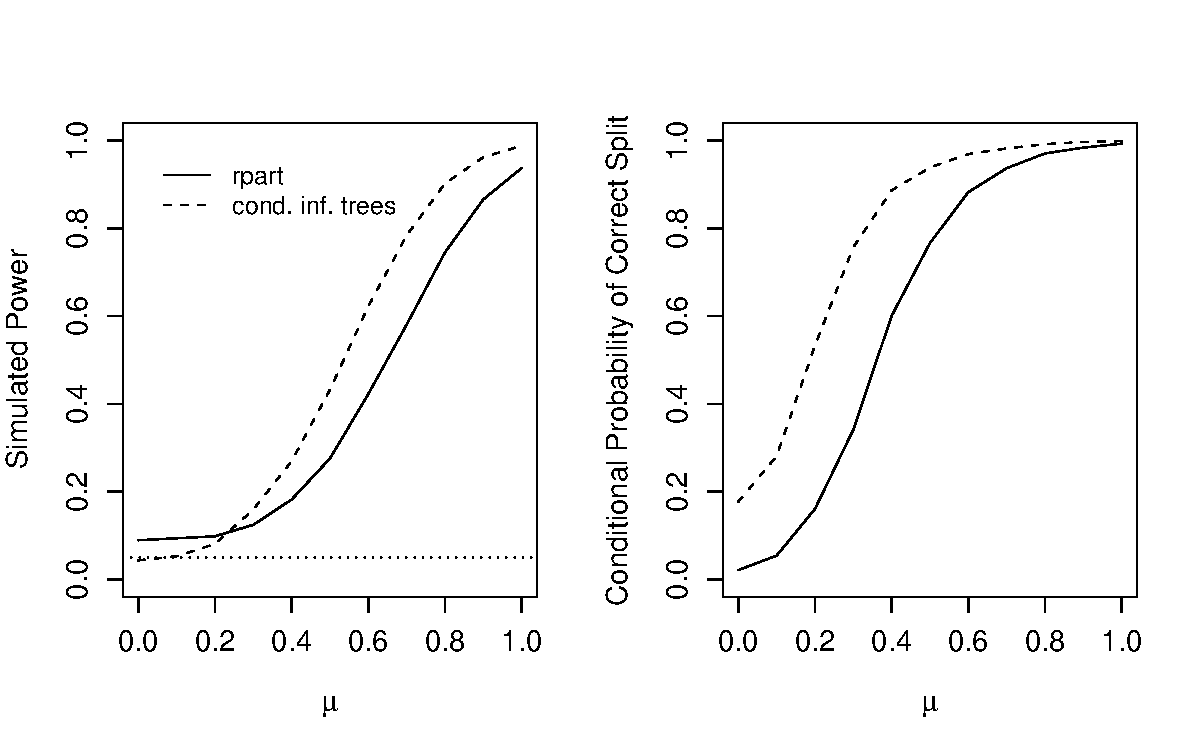
\includegraphics[width = \textwidth]{power_split}
\caption{Simulated power, i.e. the probability of a root split (left), and the simulated
         conditional probability of a correct split in variable $X_6$ given
         that any root split was established (right) are displayed. The 
         dotted horizontal line represents $\alpha = 0.05$.
         The results are based on 10,000 replications. \label{power}}
\end{center}
\end{figure}

The advantageous properties of the conditional inference trees are obvious
for the simple simulation model with one split only. We now extend our
investigations to a simple regression tree with four terminal nodes. The
response variable is normal with mean $\mu$ depending on the covariates as
follows:
\begin{eqnarray} \label{part}
\Y \sim \left\{ \begin{array}{ll} 
             \mathcal{N}(1,1) & \text{if } X_6 = 0 \text{ and } X_1 < 0.5 \\
             \mathcal{N}(2,1) & \text{if } X_6 = 0 \text{ and } X_1 \ge 0.5 \\
             \mathcal{N}(3,1) & \text{if } X_6 = 1 \text{ and } X_2 < 0.5 \\
             \mathcal{N}(4,1) & \text{if } X_6 = 1 \text{ and } X_2 \ge 0.5.
            \end{array} \right.
\end{eqnarray}

We will focus on two closely related criteria describing the partitions
induced by the algorithms: the complexity of the induced partitions and the
structure of the trees. 
The number of terminal nodes of a tree 
is a measure of the complexity of the model and can easily be compared with
the number of cells in the true data partition defined by (\ref{part}). 
However, the appropriate complexity of a tree does not ensure that the
tree structure describes the true data partition well. 
Here, we measure the discrepancy between the true data partition and 
the partitions obtained from recursive partitioning by the
normalized mutual information \citep[`NMI', ][]{StrehlGhosh2002}, essentially
the mutual information of two partitions standardized by the
entropy of both partitions. Values near one indicate similar to equal   
partitions while values near zero are obtained for structurally different
partitions.

For 1,000 learning samples of size $n = 100$ drawn from the simple tree model,
Table \ref{nodes} gives the cross-tabulated
number of terminal nodes of conditional inference trees and pruned
exhaustive search trees computed by \texttt{rpart}. The null hypothesis of
marginal homogeneity for ordered variables \citep{Agresti2002} 
can be rejected ($P\text{-value} <
0.0001$) indicating that the partitions obtained from both algorithms differ
with respect to the number of terminal nodes.
Conditional inference trees select a right-sized tree (four
terminal nodes) in $78.7\%$ of the cases while \texttt{rpart} generates
trees with four terminal nodes for $63.7\%$ of the learning samples. 
In general, pruning as
implemented in \texttt{rpart} tends to produce trees with a larger number of
terminal nodes in this example. 

\begin{table}
\begin{center}
\begin{tabular}{lrrrrrrr|r}
      & \multicolumn{6}{r}{Conditional Inference Trees} & \\
& & 2 & 3 & 4 & 5 & 6 & $\ge$ 7 & \\
& 2 & 3 & 4 & 5 & 0 & 0 & 0 & 12 \\
& 3 & 0 & 48 & 47 & 3 & 0 & 0 & 98 \\
\texttt{rpart} & 4 & 0 & 36 & 549 & 49 & 3 & 0 & 637 \\
& 5 & 0 & 12 & 134 & 25 & 1 & 0 & 172 \\
& 6 & 2 & 6 & 42 & 10 & 1 & 0 & 61 \\
& $\ge$ 7 & 0 & 3 & 10 & 6 & 1 & 0 & 20 \\ \hline
 &  & 5 & 109 & 787 & 93 & 6 & 0 & 1000 \\
\end{tabular}
\caption{Number of terminal nodes for \texttt{rpart} and conditional
         inference trees when the learning sample is actually partitioned into four
         cells. \label{nodes}}
\end{center}
\end{table}

The correct tree structure with four leaves, with the first split in $X_6$ and splits in
$X_1$ and $X_2$ in the left or right node, is detected by \texttt{rpart} in
$63.3\%$ of the simulation runs and in $77.5\%$ of the cases by conditional
inference trees. The NMI measure between the true partition of the data given by (\ref{part})
and the partitions induced by the tree algorithms needs to be compared for
instances with informative NMI measures only, i.e., the cases
where the NMI between \texttt{rpart} and the true data partition and the NMI
between conditional inference trees and the true data partition coincide do
not cover any information. A
density estimate of the NMI difference between partitions obtained from
\texttt{rpart} and
conditional inference tree partitions in Figure \ref{density} shows that the
partitions induced by conditional inference trees are, one average, closer
to the true data partition. 

\begin{figure}[t]
\begin{center}
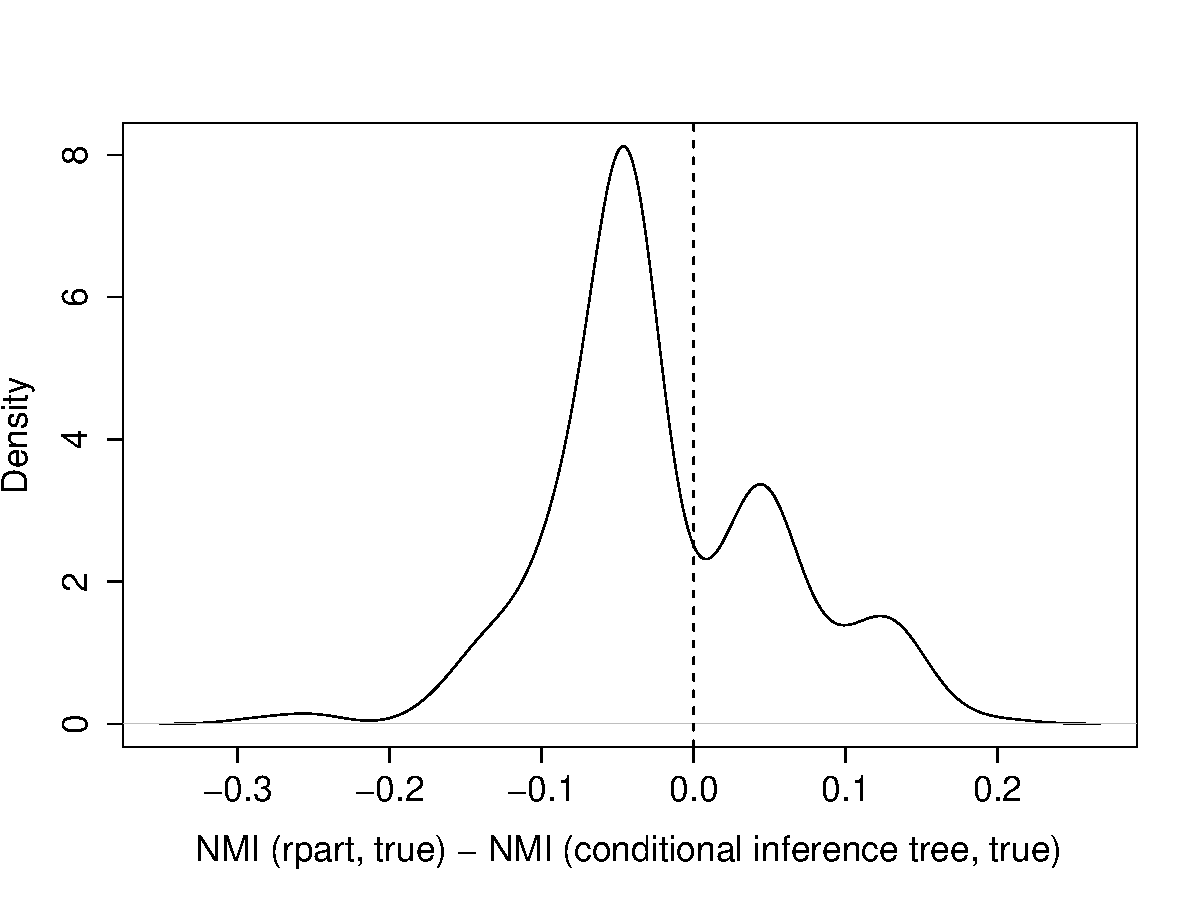
\includegraphics[width = \textwidth]{nmisim}
\caption{Density estimate of the difference in normalized mutual information
         of the true partition and the partitions induced by \texttt{rpart}
         and conditional inference trees. Instances with a NMI difference of
         zero were excluded -- the results are based on $394$ 
         replications. \label{density}}
\end{center}
\end{figure}


\paragraph{Prediction Accuracy.}

Assertion 3) is investigated by means of $11$ benchmarking problems from
the UCI repository \citep{Blake+Merz:1998} as well as the glaucoma data (see
Section \ref{illustrations}).
Characteristics of the problems are given in Table~\ref{benchdata}. We draw
$500$ random samples from the out-of-bag performance measures
(misclassification or mean-squared error) in a dependent $K$-sample design
as described in the conceptual framework for benchmark experiments of 
\cite{Benchmarking2005}. 

\begin{table}[t]
\begin{center}
\begin{tabular}{lrrrrrrr}
               & $J$ & $n$   & NA  & $m$  & nominal & ordinal & continuous \\ \hline
Boston Housing & -- & 506 & --  & 13 & --       & --       & 13    \\
Ozone          & -- & 361 & 158 & 12 & 3      & --       & 9     \\
Servo          & -- & 167 & --  & 4  & 4       & --       & -- \\ \hline
Breast Cancer  & 2 & 699 & 16 & 9  & 4       & 5       & --     \\
Diabetes       & 2 & 768 & --  & 8  & --       & --       & 8     \\
Glass          & 6 & 214 & --  & 9  & --       & --       & 9     \\
Glaucoma       & 2 & 196 & --  & 62 & --       & --       & 62    \\
Ionosphere     & 2 & 351 & --  & 33 & 1       & --       & 32    \\
Sonar          & 2 & 208 & --  & 60 & --       & --       & 60    \\
Soybean        & 19 & 683 & 121 & 35 & 35    & 5       & --     \\
Vehicle        & 4  & 846 & -- & 19 & --       & --       & 19    \\
Vowel          & 11 & 990 & -- & 10 & 1       & --       & 9     \\
\end{tabular}
\caption{Summary of the benchmarking problems showing the number of classes
of a nominal response $J$ (`--' indicates a continuous response), the number
of observations $n$, the number of observations 
with at least one missing value (NA) as well as the measurement
scale and number $m$ of the covariates. \label{benchdata}}
\end{center}
\end{table}


The performance of conditional inference trees is compared to the
performance of exhaustive search trees with pruning (as implemented in
\texttt{rpart}) and unbiased \texttt{QUEST} trees (nominal responses) and
piecewise constant \texttt{GUIDE} trees (numeric responses), respectively.
The tree sizes for \texttt{QUEST} and \texttt{GUIDE} are determined by
pruning as well.

Two performance distributions are said to be equivalent when 
the performance of the conditional inference trees compared 
to the performance of one competitor (\texttt{rpart}, \texttt{QUEST} or \texttt{GUIDE}) 
does not differ 
by an amount of more than $10\%$. The null hypothesis of non-equivalent performances 
is then defined in terms of the ratio of the expectations of the performance
distribution of conditional inference trees and its competitors. 
Equivalence can be established at level $\alpha$ based on two one-sided level
$\alpha$ tests by the intersection-union principle \citep{BergerHsu1996}.
Here, this corresponds to a rejection of the null hypothesis of
non-equivalence performances at the $5\%$ level when the $90\%$ two-sided
\cite{Fieller1940} confidence interval 
for the ratio of the performance expectations is completely included in the 
equivalence range $(0.9, 1.1)$.

%%The distribution of the performance ratios between conditional inference
%%trees and \texttt{rpart} trees together with the Fieller confidence intervals are
%%depicted in Figure~\ref{ratiofig}. The corresponding plot for the comparison
%%of conditional inference trees and \texttt{QUEST}/\texttt{GUIDE} is given in
%%Figure \ref{ratiofigQG}.

\begin{figure}[t]
\begin{center}
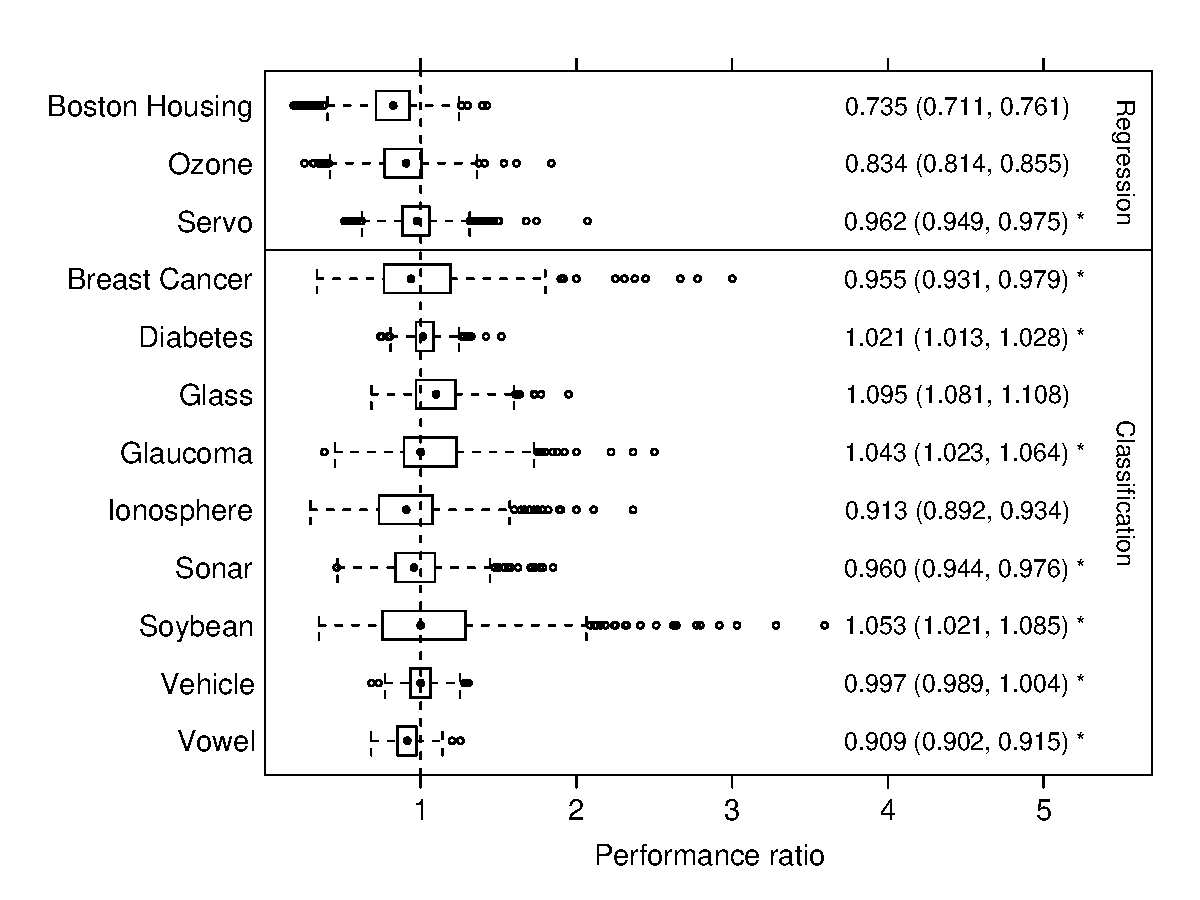
\includegraphics[width = \textwidth]{ratiobox}
%Z%  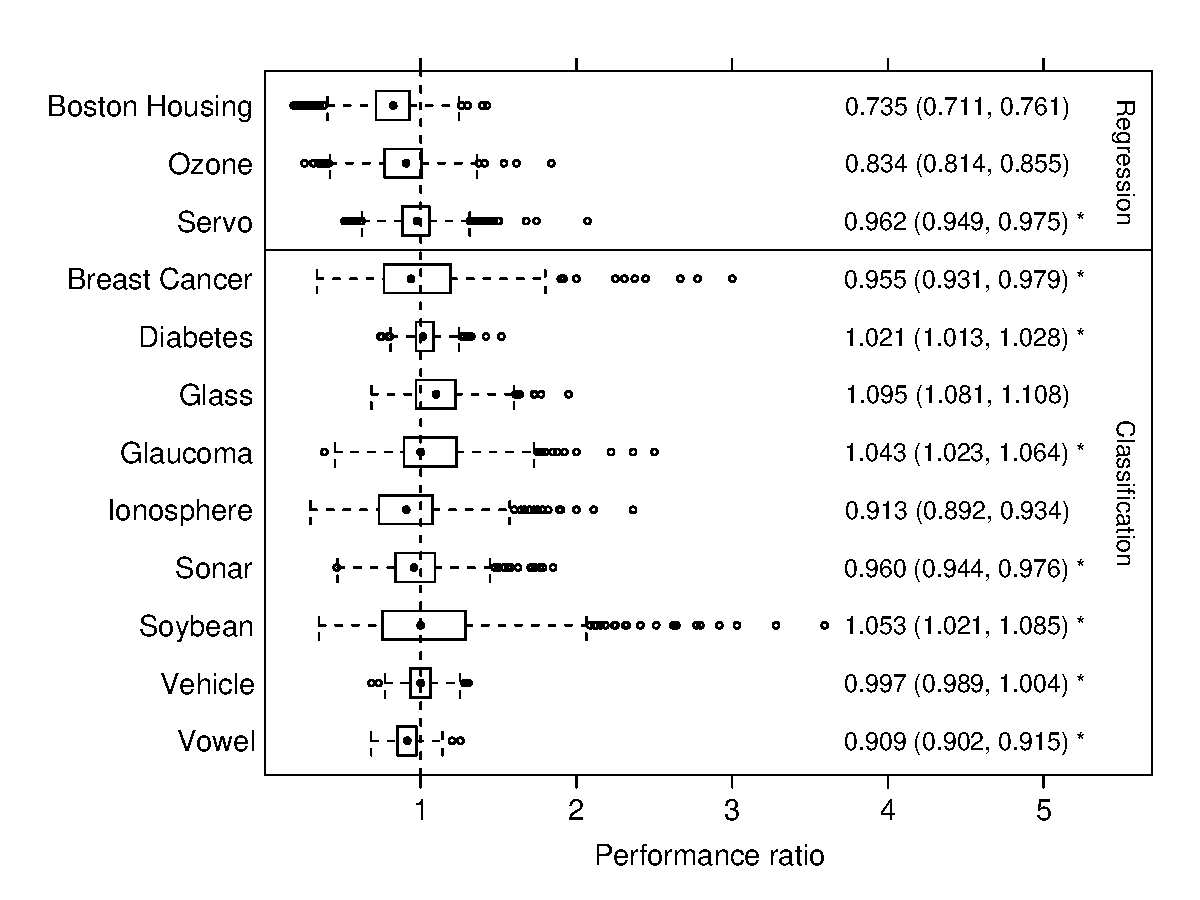
\includegraphics[width = 14cm]{ratiobox}
\caption{Distribution of the pairwise ratios of the performances of the
         conditional inference trees and
         \texttt{rpart} accomplished by estimates and $90\%$ Fieller confidence intervals for
         the ratio of the expectations of the performance distributions. 
         Stars indicate equivalent performances, i.e., the confidence interval 
         is covered by the equivalence range $(0.9, 1.1)$.\label{ratiofig}}
\end{center}
\end{figure}

\begin{figure}[t]
\begin{center}
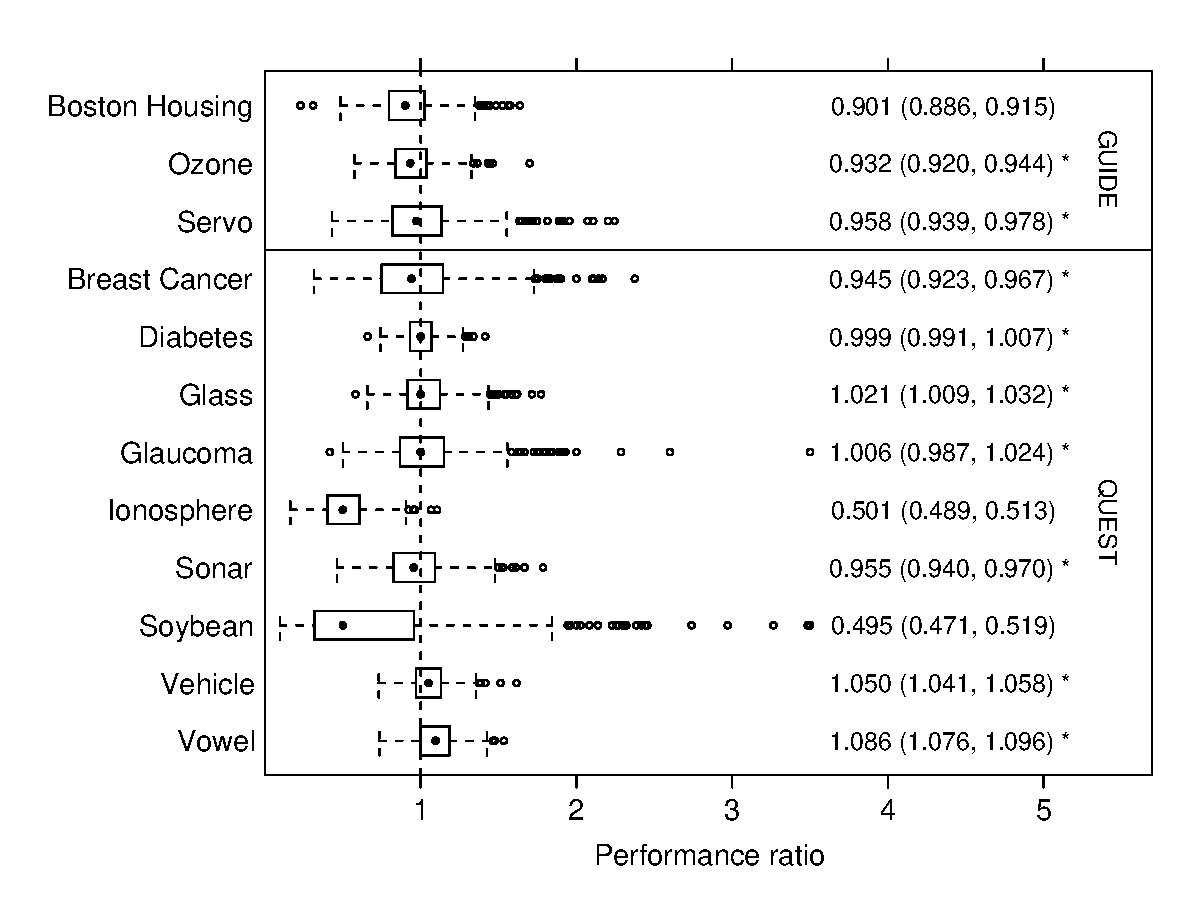
\includegraphics[width = \textwidth]{ratioboxQUEST_GUIDE}
\caption{Distribution of the pairwise ratios of the performances of the
         conditional inference trees and
         \texttt{QUEST} (classification) or \texttt{GUIDE} (regression) 
         accomplished by estimates and $90\%$ Fieller confidence intervals for
         the ratio of the expectations of the performance distributions. 
         Stars indicate equivalent performances, i.e., the confidence interval 
         is covered by the equivalence range $(0.9, 1.1)$.\label{ratiofigQG}}
\end{center}
\end{figure}


The boxplots of the pairwise ratios of the performance measure evaluated for
conditional inference trees and pruned exhaustive search trees
(\texttt{rpart}, Figure \ref{ratiofig}) and pruned unbiased trees 
(\texttt{QUEST}/\texttt{GUIDE}, Figure \ref{ratiofigQG}) are accomplished by
estimates of the ratio of the expected performances and corresponding
Fieller confidence intervals. For example, an estimate of the ratio 
of the misclassification errors 
of \texttt{rpart} and conditional inference trees for the glaucoma data of
$1.043$ means that the misclassification error of conditional inference
trees is $4.3\%$ larger than the misclassification error of \texttt{rpart}.
The confidence interval of $(1.023, 1.064)$ leads to the conclusion that
this inferiority is within the pre-defined equivalence margin of
$\pm 10\%$ and thus the performance of conditional inference trees is on par
with the performance of \texttt{rpart} for the glaucoma data.

\begin{figure}[t]
\begin{center}
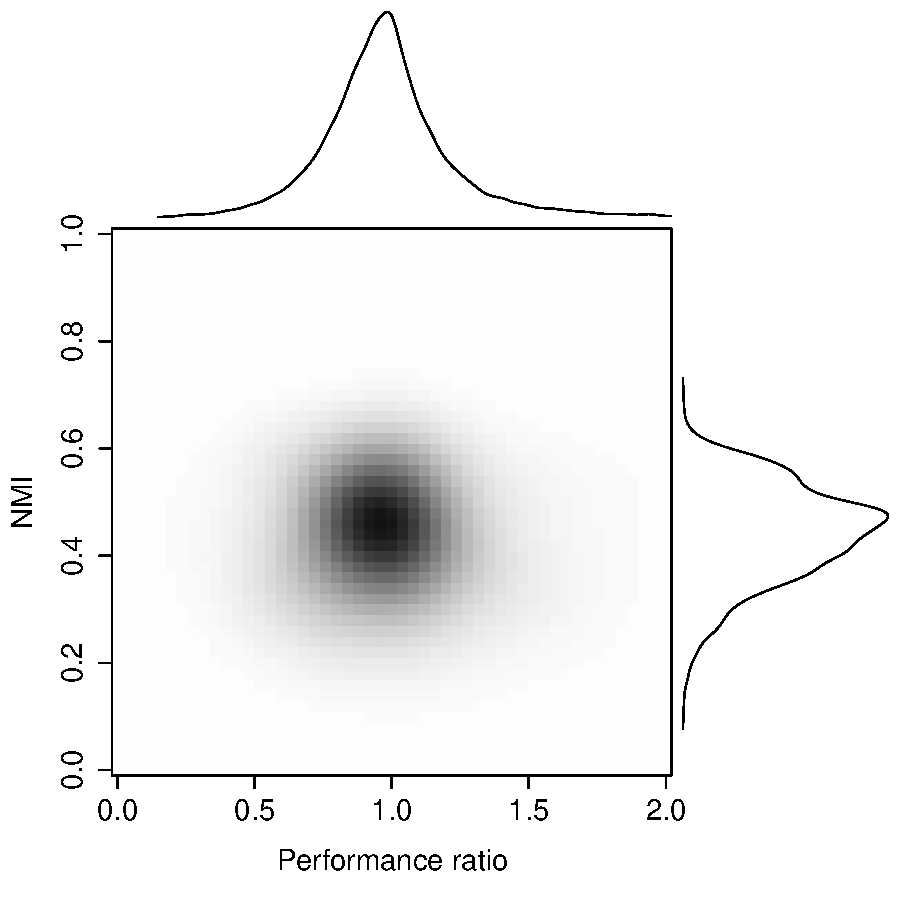
\includegraphics[width = 12cm]{nmiratiodens}
\caption{Distribution of the pairwise performance ratios of conditional
         inference trees and \texttt{rpart} and the normalized mutual
         information measuring the discrepancy of the induced partitions. 
         \label{densfig}}
\end{center}
\end{figure}


Equivalent performance between conditional inference trees and
\texttt{rpart} cannot be postulated for the Glass data. The
performance of the conditional inference trees is
roughly $10\%$ worse compared with \texttt{rpart}. In all other cases, the
performance of conditional inference trees is better than or equivalent to the
performance of exhaustive search (\texttt{rpart}) and unbiased procedures
(\texttt{QUEST} or \texttt{GUIDE}) with pruning.
The conditional inference trees 
perform better compared to \texttt{rpart} trees by a magnitude of $25\%$ (Boston
Housing), $10\%$ (Ionosphere) and $15\%$ (Ozone). The improvement upon
unbiased \texttt{QUEST} and piecewise constant \texttt{GUIDE} models 
is $10\%$ for the Boston Housing data and $50\%$ for the
Ionosphere and Soybean data.
For all other problems, the performance of conditional inference trees 
fitted within a permutation testing framework can
be assumed to be equivalent to the performance of all three competitors. 

The simulation experiments with model (\ref{part}) presented in the first
paragraph on estimation accuracy lead to the impression
that the partitions induced by \texttt{rpart} trees are structurally
different from the partition induced by conditional inference trees. Because
the `true' partition is unknown for the datasets used here, we
compare the partitions obtained from conditional inference trees and
\texttt{rpart} by their normalized mutual information.
The median normalized mutual information is  
$0.447$ and a bivariate density estimate depicted in
Figure~\ref{densfig} does not indicate any relationship between the ratio of
the performances and the discrepancy of the partitions. 

This results is interesting from a practical point of view. 
It implies that two recursive partitioning
algorithms can achieve the same prediction accuracy but, at the same time,
represent structurally different regression relationships, i.e., 
different models and thus may lead to different conclusions about the 
influence of certain covariates on the response.
